\begin{frame}{Collaboration Initiative}

  \begin{center}
    Мысли глобально, действуй локально

    
\includegraphics[height=0.6\textheight]{think-globally-act-locally}

    \begin{itemize}
      \item Инициатива сотрудников снизу
      \item Работаем через нейтральную открытую площадку
    \end{itemize}

  \end{center}

\end{frame}

\begin{frame}{Конкуренция между компаниями}
      
  \center\Large\alert{Конкуренции - нет}\footnote{См кол-во проектов и падение плотности специалистов}

  \center
\includegraphics[height=0.7\textheight]{penguin}

\end{frame}


\begin{frame}[fragile]{Ранняя публикация результатов}

  \begin{center}
    \alert{Release early, release offen} 

\begin{lstlisting}
  # find linux_courses/ -name "*.tex"|wc -l
  48
\end{lstlisting}

    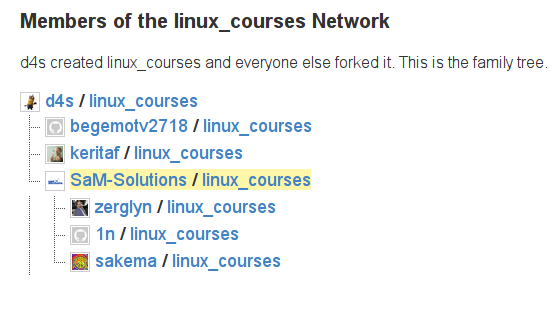
\includegraphics[width=0.65\textwidth]{members}

    \alert{Go github!}
  \end{center}
  
\end{frame}

\begin{frame}{Call for partnership}
  
  \begin{center}
    Открытый проект 'Linux образование' предлагает воспользоваться имеющимися материалами.
    
    
\includegraphics[width=0.6\textwidth]{copying}
  \end{center}

  А также с благодарностью примет:
  \begin{itemize}
    \item на хранение, распространение и доработку курсы
      \begin{itemize}
	\item незаконченные и готовые
	\item одноразовые и умершие
	\item осиротевшие
      \end{itemize}
    \item патчи
    \item баг-репорты
    \item pull-request'ы
  \end{itemize}

\end{frame}
